\section{Research Method}

We adopted Grounded Theory (GT) as research method. GT is a method originally
proposed in \cite{glase1967discovery} which has as distinguishing features the
absence of clear research hypothesis upfront and limitation of literature
exposure at the beginning of the research. Is a theory-developing approach in
contrast with the more traditional theory-testing approach
\cite{coleman2007using}.

Some of related work claimed to used "GT inspired" approaches. It is a very
common rhetoric in recent research on software engineering, but only research
that embodies GT’s core principles should claim to be a grounded theory study
\cite{stol2016grounded}.

GT was employed as the research method for the following reasons:
\begin{itemize}

\item GT is a consolidated method in other areas of research like sociology,
nursing, education and finances and is increasingly being employed
to study software engineering topics \cite{stol2016grounded};

\item GT is considered an adequate approach to investigate scenarios with
questions such as \textit{what's going on here?} \cite{barnsteiner2002using},
which is exactly the scenario proposed here: what's going on DevOps adoption?

\item GT allows the researcher to get descriptions without bias of previous
researches, which is adequate to collect empirical evidence directly from the
practice on industry. The evidence is only reintegrated back with literature
after the theory construction.

\end{itemize}

Since the publication of the original version in \cite{glase1967discovery},
several modifications and variations occurred in the original text, coming to
exist at least seven different versions of the method \cite{denzin2007grounded},
where the main versions are those of Glaser or classic, Strauss and
Charmaz \cite{stol2016grounded}. The study presented in \cite{stol2016grounded}
explores the main aspects of GT versions and establishes that GT studies has to
specify which version is used on it. In our study, we choose the classic
version. The first reason to our choice is that we did not have a research
question at the beginning of the research, exactly as suggested in the classic
version, we start from a interest area that are: successfully DevOps adoption
in industry. And the second reason is because the more detailed papers in
software engineering research use predominantly this version
\cite{stol2016grounded}.

\subsection{GT Procedures}

In Fig. \ref{fig1}, reproduced from \cite{adolph2011using}, is showed the view
of the grounded theory procedures that we followed in the conduction of this
research.

\begin{figure}[htpb]
  \centering
  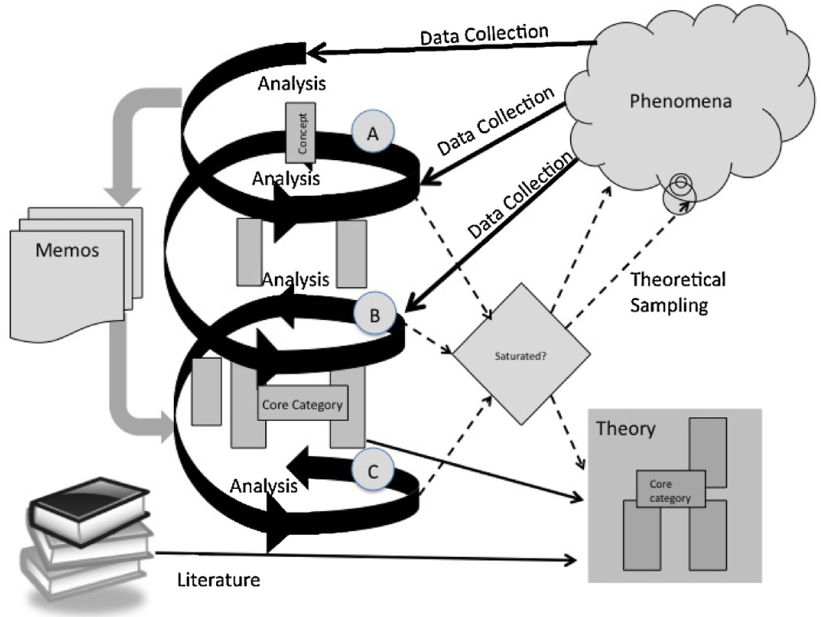
\includegraphics[width=0.5\textwidth,natwidth=821,natheight=617]{GT.png}
  \caption{The GT Method \cite{adolph2011using}}
  \label{fig1}
\end{figure}

\begin{enumerate}[label=(\Alph*)]
\item Initially, we begin collecting data about the adoption process from
companies that have successfully adopted it. As the data were collected, they
were also analyzed simultaneously. The raw data is analyzed by searching for
patterns of incidents to indicate concepts, and concepts grouped into
categories. This first step, where all raw data is analyzed, is called open
coding \cite{stol2016grounded}.

\item The categories are developed by constant comparison of new incidents with
previous. Every grounded theory study has to identify a "core category"
\cite{stol2016grounded}. The core category is responsible for enabling the
integration of the other categories and structuring the results into a dense
and consolidated grounded theory \cite{jantunen2014using}. The identification
of the core category represents the end of open coding and the beginning of the
selective coding. In selective coding, only specific variables that are
directly related to the core category and their relationships are coded, in
order to enable the production of a harmonic theory \cite{coleman2007using}
\cite{hoda2011impact}.

\item After saturation, the resulting theory is reintegrated back into
literature comparing with existing theories. The literature search is performed
only later to avoid forcing preconceived concepts on the theory development
\cite{adolph2012reconciling}.

\item Throughout the process, memos are wrote capturing thoughts and analytic
processes; the memos support the emerging concepts, categories, and their
relationships \cite{adolph2012reconciling}.

\end{enumerate}

The following sub-sections present details of procedures applied in this study,
containing some examples to illustrate their application.

\subsection{Data Collection}
We conducted semi-structured interviews with 15 practitioners of companies from
Brazil, Portugal, Ireland, United States and Spain. This practitioners claim
to have participated to DevOps adoption process in your companies. Participants
were recruited through direct contact in DevOps days event and some general
calls for participation posted on DevOps user groups, social networking sites
and local communities. A variety of company types were covered in order to
achieve a heterogeneous perspective, increasing the potential of generalization
of the results. \ref{participant_table} presents the participant
characteristics.


\begin{table}[t]
\centering
\caption{Participant Profile}
\label{participant_table}
\begin{tabular}{ccccccc}
\textbf{P\#}          & \textbf{Role}         & \textbf{SWX} & \textbf{DX} & \textbf{CN}   & \textbf{Domain}    & \multicolumn{1}{l}{\textbf{CS}} \\
P1                   & DevOps Developer      & 9            & 2           & IR            & IT                 & S                               \\

P2                   & DevOps Consult.       & 9            & 3           & BR            & IT                 & M                               \\

P3                   & DevOps Developer      & 8            & 1           & IR            & IT                 & S                               \\

P4                   & Computer Tech.        & 10           & 2           & BR            & Health             & S                               \\

P5                   & Systems Engineer      & 10           & 3           & SP            & Telecom            & XL                              \\

P6                   & Developer             & 3            & 1           & PO            & IT                 & S                               \\

P7                   & Support Analyst       & 15           & 2           & BR            & Telecom            & L                               \\

P8                   & DevOps Engineer       & 20           & 9           & BR            & Imob?              & M                               \\

P9                   & IT Manager            & 14           & 8           & BR            & IT                 & M                               \\

P10                  & Network Admin.        & 15           & 3           & BR            & IT                 & S                               \\

P11                  & Embras                & 0            & 0           & BR            & *                  & *                               \\

P12                  & Sprinklr              & 0            & 0           & US            & *                  & *                               \\

P13                  & IFood                 & 0            & 0           & BR            & *                  & *                               \\

P14                  & IT Manager            & 0            & 0           & BR            & *                  & *                               \\

P15                  & Daniel Almeida        & 0            & 0           & BR            & *                  & *
\end{tabular}
\end{table}

The first column refers to participant numbers P1-P15 to maintain anonymity in
conformance with the human ethics guidelines. The second column the role of
each participant in your respective company. The remain columns list their
years of total experience in software development (SWX), years of experience
with DevOps (DX), country of work (CN), main domain of the company, and company
sizes (CS).

The interview were conducted over one year using Skype calls and lasted
approximately 30 minutes on average.

Data collection and analysis were iterative so the collected data helped guide
future interviews. The questions of interview evolved according to the progress
of the research...

\subsection{Data Analysis}
The interviews were voice recorded, transcribed, and analyzed. The first moment
of the analyze, called open coding in GT, started immediately after
transcription of the first interview. So the results of the analyze of the
first interview already server to evolve the interview script to the second and
so on.

The open coding lasted until there was no doubt about the core category of the
study. Similar to the described \cite{adolph2012reconciling} we have started
with a strong candidate to core category that has not been consolidated. Until
the analyze of the four interview, we have cogitated automation as core
category because it is a recurring pattern in our data. But, we quickly
realized that the "automation" category did not explain most of the behaviors
or events in our data. At the same time we start to perceive that the
collaboration culture also appeared recurrently in the analysis and with more
potential to explain the remaining events. We then started to ask explicitly
about the role of the automation and how to the collaboration culture is formed
in a DevOps adoption process.

After the adaptations made in the script and analysis of new data in a constant
comparison process, taking into account the previous analyses and the
respective memos wrote during all the process, in the analysis of the tenth
interview, we concluded that was unequivocal the core role of the
category "collaboration culture" in the explanation about how DevOps was
successfully adopted in the companies. At this moment, the open coded ended
and the selective coding started.

After the discovery of the core category, we start to restrict the coding only
to specific variables that are directly related to the core category and their
relationships: the selective coding.

With more three interviews and respective analyze, we started to realize that
the new data added less and less content to the emerging theory. The
explanation around how the collaboration culture is developed providing
DevOps adoption showed signs of saturation. We then conducted more two
interviews to conclude that we had reached the theoretical saturation.

After saturation, we start the theoretical coding to find a way to integrate
all the concepts, categories and memos in the form of a cohesive and
homogeneous theory, where we have pointed out the role of the categories as
enablers and outcomes, as shown above.

To illustrate the coding procedures, we present an example of working from
interview transcript to the findings for one of the categories: automation.

Apresentar aqui a exemplificacao da codificacao....

\subsection{Reintegrate }
